\section{Overview}
\label{sec: overview}%
In this section, a general description of the architecture of the \verb|CKB| system is provided.
The main aspects of the design are:
\begin{itemize}
    \item \textbf{Client-Server architecture. } It consists of a presentation tier, an application and a data tier.
    The firsts one allow the user to communicate with the server and shows him through the UI the answers it receives back from the application tier.
    The second one receives requests from users, elaborates answers, changes the status communicating with the data tier and sends back the needed information to users.
    Finally, the data tier stores, updates, and handles the information.
    \item \textbf{Microservices. } Functionalities of the system are divided into several services in order to reduce dependencies between
    modules and to increase scalability, availability and maintainability of the system.
\end{itemize}

\newpage
\section{Component View}
\label{sec: component_view}%
The UML component diagram shows all the identified components in the \verb|CKB| system.
It also describes the relations between the modules, representing the verse of the communication flow and the actors participating.
It is divided into a WebApplication, which is the front-end for users, and a back-end, composed of the \verb|CKB Core Business Logic| and the \verb|CKB Notification System|.
External entities to which the system holds a dependency are also shown.

\subsection{Component diagram}
\label{subsec:component_diagram}%
\begin{figure} [H]
    \begin{center}
        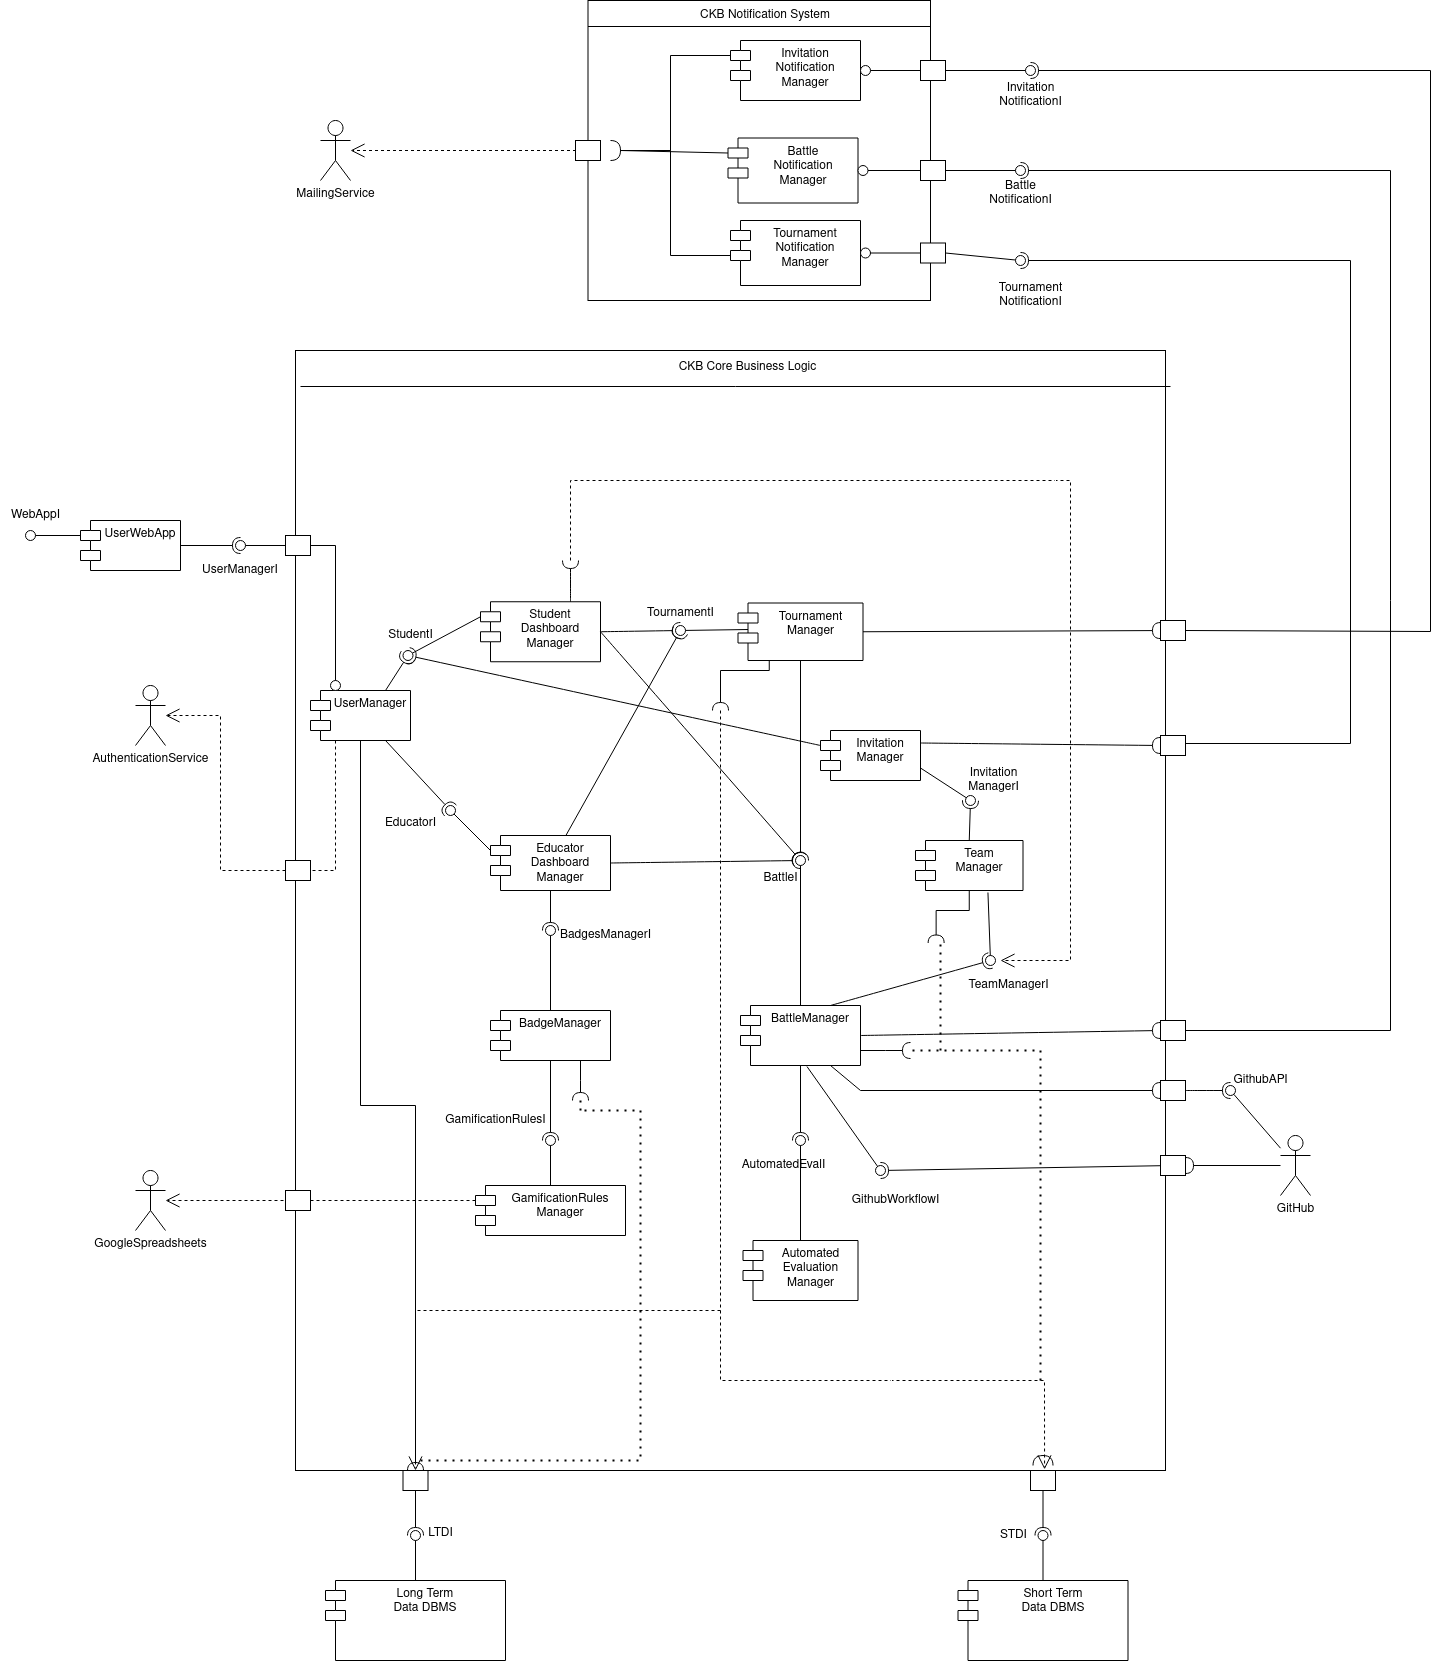
\includegraphics[width=1\linewidth]{Images/compdiag.png}
        \caption{Component diagram of the CKB platform.}
        \label{fig: cd}
    \end{center}
\end{figure}

\newpage
\subsection{Components description}
\label{subsec:components_description}%
The components are:
\begin{itemize}
    \item \textbf{User WebApp.} \verb|User| \verb|WebApp| is the front-end for users. 
    %It allows them to interact with the system by offering the following functions through the interface UserAppI:
    %    \begin{itemize}
    %        \item \textbf{Register} 
    %        \item \textbf{Login} 
    %        \item \textbf{A} 
    %        \item \textbf{Z} 
    %        \item \textbf{Z} 
    %        \item \textbf{Z} 
    %        \item \textbf{Z} 
    %        \item \textbf{Z} 
    %    \end{itemize}

    %PROBABILMENTE UserManager SARÀ DA CAMBIARE E/O APPROFONDIRE MENTRE FAREMO LA SEZIONE Component Interfaces
    %IDEM PER UserWebApp
    \item \textbf{UserManager.} \verb|UserManager| component offers, through the interface \verb|UserManagerI|, the basic function for handling users:
        \begin{itemize}
            \item \textbf{Register}
            \item \textbf{Login}
            %tanta altra roba di sicuro
        \end{itemize}
        It also provides user information to the \verb|EducatorDashboardManager| component and the \verb|StudentDashboardManager| component depending on the role of the logged user.
    \item \textbf{Educator Dashboard Manager.} \verb|Educator| \verb|Dashboard| \verb|Manager| handles the main functionalities accessible by an Educator. 
    It allows creating and managing both CodeKataBattles and Tournaments, defining new badges and rules and performing all the operations that an Educator should be able to perform according to the RASD.
    \item \textbf{Badge Manager.} \verb|Badge| \verb|Manager| is used to manage badges, allowing to perform operations such as assigning a badge to a Student, creating new badges and defining new rules and variables to obtain them.
    \item \textbf{Gamification Rules Manager.} \verb|Gamification| \verb|Rules| \verb|Manager| is used to manage rules and variables used to determine winners of badges. 
    This component relies on an external actor, Google Spreadsheet, to allow defining new rules in a simple but effective way (Spreadsheet formulas).
    \item \textbf{Student Dashboard Manager.} \verb|Student| \verb|Dashboard| \verb|Manager| handles the main functionalities accessible by a Student.
    It allows joining and participating in CodeKataBattles and Tournaments, checking the status of the ongoing ones and the results of the past ones.
    \item \textbf{Battle Manager.} \verb|Battle| \verb|Manager| is used to manage CodeKataBattles, allowing to perform operations such as creating a new CodeKataBattle, 
    joining an existing one and checking the status of the ongoing ones through its interface \verb|BattleI|.
    \item \textbf{Tournament Manager.} \verb|Tournament| \verb|Manager| is used to manage Tournaments, allowing to perform operations such as creating a new Tournament,
    joining an existing one and checking the status of the ongoing ones through its interface \verb|TournamentI|. Educators can also add other Educators as admin to a tournament they created.
    \item \textbf{Automated Evaluation Manager.} \verb|Automated| \verb|Evaluation| \verb|Manager| is used to manage the automated evaluation of CodeKataBattles assigning scores to teams.
    \item \textbf{Team Manager.} \verb|Team| \verb|Manager| is used to manage teams, allowing to perform operations such as creating a new team, joining an existing one and inviting a student to join a team.
    \item \textbf{Invitation Manager.} \verb|Invitation| \verb|Manager| is used to manage team invitations, it is responsible for keeping track of invitations sent by Students to other Students and their status (whether they have been accepted or not).
    It communicates with \verb|TeamManager| and \verb|NotificationManager| to update teams and deliver notifications to Students.
    \item \textbf{CKB Notification System.} \verb|CKB Notification| \verb|System| allows Students to be notified via email when a new CodeKataBattle or Tournament is created or ends. It relies on an external Mailing Service. 
    This component handles notifications to be sent relying on three modules:
        \begin{itemize}
            \item \textbf{Tournament Notification Manager.} \verb|Tournament| \verb|Notification| \verb|Manager| is used to handle notifications elated to Tournament events (such as Tournament creation, registration deadline expiration and closing) 
            through its interface \verb|InvitationNotificationI|.
            \item \textbf{Battle Notification Manager.} \verb|Battle| \verb|Notification| \verb|Manager| handles notifications related to CodeKataBattles within Tournaments. It exposes an interface called \verb|BattleNotificationI| to allow the \verb|Battle Manager| 
            to deliver notifications about Battle creation, start and end to Students. 
            \item \textbf{Invitation Notification Manager.} \verb|Invitation| \verb|Notification| \verb|Manager| is used to handle notifications regarding invitations to join a team. Its interface is called \verb|InvitationNotificationI|.
        \end{itemize}
\end{itemize}
External entities are:
\begin{itemize}
    \item \textbf{Google Spreadsheet.} \verb|Google| \verb|Spreadsheets| is the engine used by Educators when creating new rules for badges. 
    \item \textbf{Mailing Service.} \verb|Mailing| \verb|Service| is used to send emails to Students when a new CodeKataBattle or Tournament is created or ends.
    \item \textbf{Github.} \verb|Github| interacts with the \verb|Battle| \verb|Manager| component to handle the code that represents the solution of a CodeKataBattle. 
    CKB platform offers APIs to allow Github Actions Workflow to trigger a pull request to the repository of the solution.
\end{itemize}
DBMS components are:
\begin{itemize}
    \item \textbf{LongTermData DBMS.} \verb|LongTermData DBMS| is the DBMS used to store and manage data that is meant to be accessed less frequently and that will probably be stored for more time, like Users, Badges, Tournament results.
    \item \textbf{ShortTermData DBMS.} \verb|ShortTermData DBMS| is the DBMS used to store and manage structured data that will probably be accessed more frequently by a higher number of users, like CodeKataBattles, Tournaments or Teams. 
    This kind of data can be stored for a shorter period of time because after the end of a Tournament or a CodeKataBattle most of it will not be useful anymore.
\end{itemize}
\section{Deployment View}
\label{sec: deployment_view}%
The distribution of components capturing the topology of the system is illustrated below by using a deployment diagram.
The system is structured in a multitier architecture.
\newline
\begin{figure} [H]
    \begin{center}
        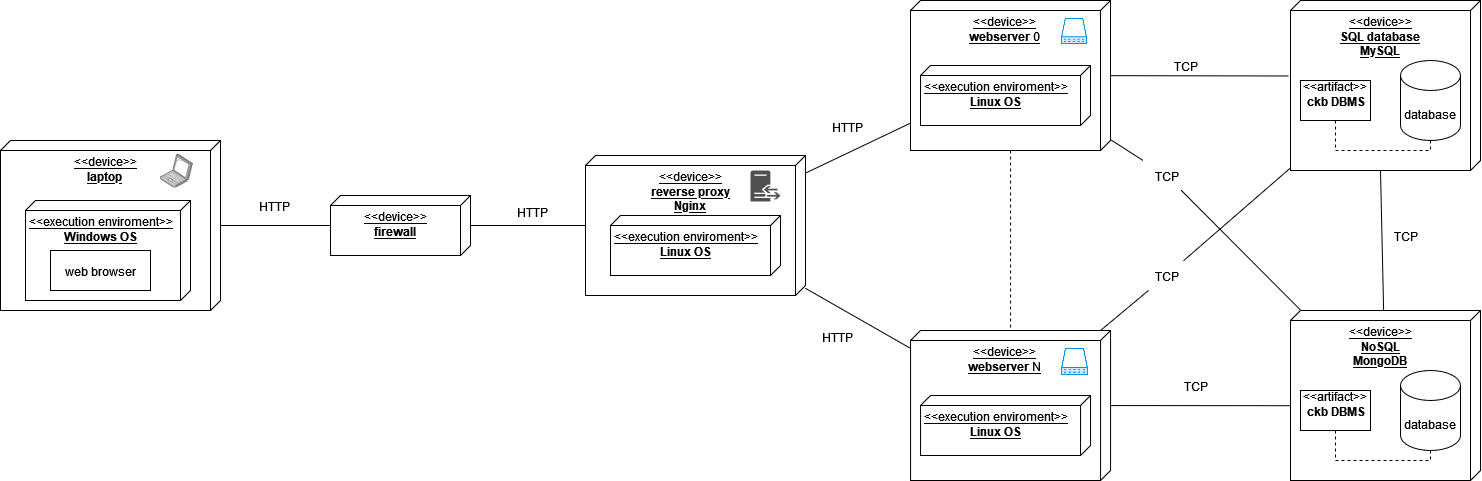
\includegraphics[width=1\linewidth]{Images/deployment_diag.png}
        \caption{Deployment diagram of the CKB platform.}
        \label{fig: depl_diagram}
    \end{center}
\end{figure}


\noindent\textbf{Laptop devices}\newline
This node represents a user's laptop, which is the client-side hardware. The "Windows OS" indicates that the laptop is running on the Windows operating system. 
The "web browser" is the software application used to access the web interface of the platform.

\noindent\textbf{Firewall}\newline
This is a security device that monitors and filters incoming and outgoing network traffic based on an organization's previously established security policies. 
Here, it acts as a barrier between secure internal networks and untrusted external networks, such as the internet.

\noindent\textbf{Reverse Proxy}\newline
This server is running Nginx, which is a web server that can also be used as a reverse proxy. This means it can distribute traffic to various servers, 
thereby acting as an additional layer of abstraction and control to smooth the flow of network traffic between clients and services.

\noindent\textbf{Webserver 0}\newline
This is one of potentially multiple web servers that handle the incoming HTTP requests from the client's web browser, process those requests, 
and serve the appropriate web pages. It runs on a Linux operating system, which suggests a preference for open-source solutions.

\noindent\textbf{Webserver N}\newline
This indicates there are multiple webservers in this deployment, following a similar configuration to "Webserver 0." 
The "N" represents an indefinite number, showing that the architecture is scalable and can include as many webservers as needed.

\noindent\textbf{SQL database (MySQL)}\newline
This database node uses MySQL, which is a relational database management system (RDBMS) based on SQL (Structured Query Language). 
It's used to store and manage the platform's structured data efficiently.

\noindent\textbf{NoSQL database (MongoDB)}\newline
This is a NoSQL database, specifically MongoDB, which is designed for storing unstructured data. It offers high performance, high availability, and easy scalability.

\noindent\textbf{ckb DBMS}\newline
This artifact within both database nodes represents the database management software that's part of the CodeKataBattle platform. It is likely the collection of schemas, 
tables, queries, reports, views, and other objects associated with the platform's database management.

\section{Component Interfaces}

\textbf{Invitation Notification Manager}
\begin{verbatim}
sendMail(n: Notification): JSONObject
listenEvent(e: InvitationEvent): boolean
updateInvitationNotification(n: set<Notification>): boolean
getNotifications(userId: Long): set<Notification>
\end{verbatim}

\textbf{Battle Notification Manager}
\begin{verbatim}
sendMail(n: Notification): JSONObject
listenEvent(e: battleEvent): boolean
updateBattleNotification(n: set<Notification>): boolean
getNotifications(userId: Long): set<Notification>
\end{verbatim}

\textbf{Tournament Notification Manager}
\begin{verbatim}
sendMail(n: Notification): JSONObject
listenEvent(e: tournamentEvent): boolean
updateTournamentNotification(n: set<Notification>): boolean
getNotifications(userId: Long): set<Notification>
\end{verbatim}

\textbf{Tournament Manager}
\begin{verbatim}
AddBadges(tId: Long, b: set<Badges>): boolean
AddBattle(tId: Long,e: Educator, b: Battle): boolean
AddStudent(tId: Long, s: Student): boolean
notifyStudents(tId: Long, e: Event): JSONObject
getBattles(tId: Long,): set<Battle>
getLeaderBoard(tId: Long,): map<int, Student>
updateLeaderBoard(tId: Long,): boolean
createTournament(e: Educator, b: set<Badges>): JSONObject
closeTournament(tId: Long,): boolean
notifyStudents(tId: Long, event: JSONObject): boolean
addEducator(tId: Long, e: Educator): boolean
getBadges(tId: Long): set<Badge>
\end{verbatim}

\textbf{Student Dashboard Manager}
\begin{verbatim}
getBadges(id: Long): set<Badge>
getTournaments(id: Long): set <Tournament>
answerInvitation(id: Long, in: InvitationNotification): boolean
getTeams(id: Long): set<Team>
\end{verbatim}

\textbf{User Manager}
\begin{verbatim}
getNotifications(id: Long): set<Notification>
deleteNotification(id: Long, n: Notification): boolean
createUser(username: String, role: userType): boolean
deleteUser(userId: Long): boolean
\end{verbatim}

\textbf{Invitation Manager}
\begin{verbatim}
sendInvitation(userId: Long, info: JSONObject): boolean
answerInvitation(userId: Long, info: JSONObject): boolean
\end{verbatim}

\textbf{Team Manager}
\begin{verbatim}
createTeam(name: String, s: set<Student>, b: Battle): boolean
addMember(tId: Long, s: Student): boolean
getMembers(tId: Long): set<Student>
getScore(tId: Long): int
setGitHubRepo(tId: Long, url: String): boolean
\end{verbatim}

\textbf{Educator Dashboard Manager}
\begin{verbatim}
getTorunaments(eId: Long): set<Tournaments>
grantPermissionToEducatorForTournament(eId: Long, tId: Long, 
                                        receiverId: Long): boolean
\end{verbatim}

\textbf{Badge Manager}
\begin{verbatim}
createBadge(rules: JSONObject): boolean
getBadge(bId: Long): Badge
getBadges(): set<Badge>
\end{verbatim}

\textbf{Battle Manager}
\begin{verbatim}
addTeam(bId: Long, t: Team): boolean
getLeaderBoard(bId: Long): map<int, Team>
updateLeaderboard(bId: Long): boolean
createBattle(e: Educator, battleInfo: JSONObject): boolean
notifyTeams(bId: Long, event: JSONObject): boolean
\end{verbatim}

\textbf{Automated Evaluation Manager}
\begin{verbatim}
evaluateTeam(b: Battle, t: Team): int
\end{verbatim}

\textbf{Gamification Rules Manager}
\begin{verbatim}
createRule(rule: JSONObject): boolean
createVariable(var: JSONObject): boolean
getRules(): JSONObject
getVariables(): JSONObject
\end{verbatim}


    



\section{Runtime View}
\label{sec:runtime_view}%
Here we present the dynamic of our system through sequence diagrams.
We have found the components that communicate with each other to form our system, so now we explain their behaviors.

First, we will present CKB platform actions from the point of view of a general user, i.e., logging in, booking a charge, managing his profile, etc.
Then, we will present CKB platform actions from the point of view of the student and educator, actions that are related to their specific role.
In this section, we hadn't presented all the RASD document use cases because we have decided to focus on the critical part of the system functionalities.

\paragraph{Registered User Login}
When a user WebApp wants to log in to the CKB platform, he calls the ``\verb|logIn|'' function from the \verb|UserManager| component through it's interface.
The \verb|UserManager| component then requests the UserWebApp to display the login form from which, after the user inserted the credentials it sends the information to the
\verb|AuthenticationService| to validate it's correctness. Based on the response from the \verb|AuthenticationService| the \verb|UserManager| component will send a confirmation or an error to the client.

\begin{figure}[H]
    \begin{center}
        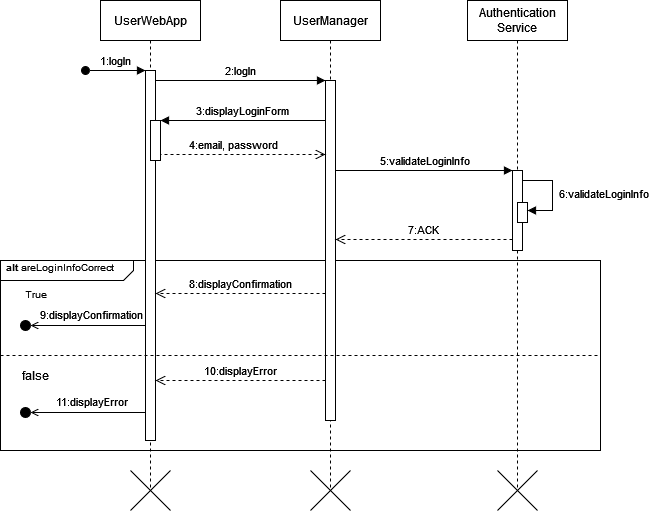
\includegraphics[width=\linewidth]{Images/sequence/Sd_login.png}
        \caption{Registered User logs in sequence diagram}
        \label{fig:user_logs_in}
    \end{center}
\end{figure}

\paragraph{Student subscribe to a tournament}
When a student wants to subscribe to a open tournament, the User WebApp after login knows that the user is a student so it shows the student the corresponding StudentDashboard.
In the StudentDashboard the student can select a tournament through the list of tournaments and clicks the subscribe button near the selected tournament.
With the interface \verb|TournamentI| the \verb|StudentDashboardManager| calls the subscribe function, the \verb|TournamentManager| will check if in the CKB data base the student has already subscribed.
Only then the \verb|TournamentManager| will sends a corresponding confirmation or an error to the client.

\begin{figure}[H]
    \begin{center}
        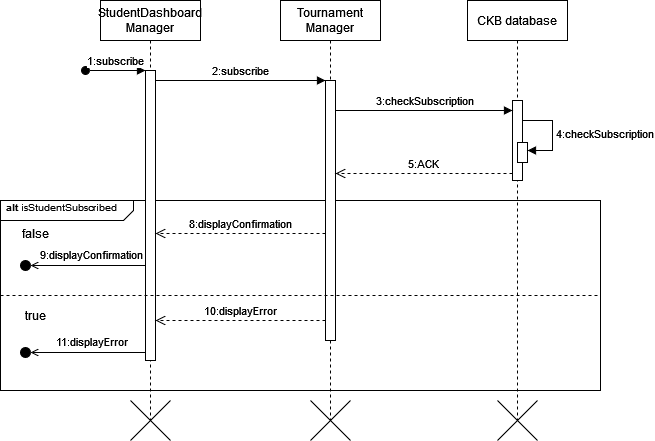
\includegraphics[width=\linewidth]{Images/sequence/Sd_subscription.png}
        \caption{Student subscribe sequence diagram}
        \label{fig:student_subscribe}
    \end{center}
\end{figure}


\paragraph{Student creates a team}
For students already subscribed in a tournament, they can call the \verb|createTeam| function through the \verb|TeamManagerI| interface.
\verb|TeamManager| component will send a request to the \verb|StudentDashboardManager| for the size and name of the group. After the student has inputed the information, the \verb|TeamManager|
will check the CKB database to ensure there are no teams with the same name already inside the DB. Then it will create the Team and norificate the student of the success or send an error.


\begin{figure}[H]
    \begin{center}
        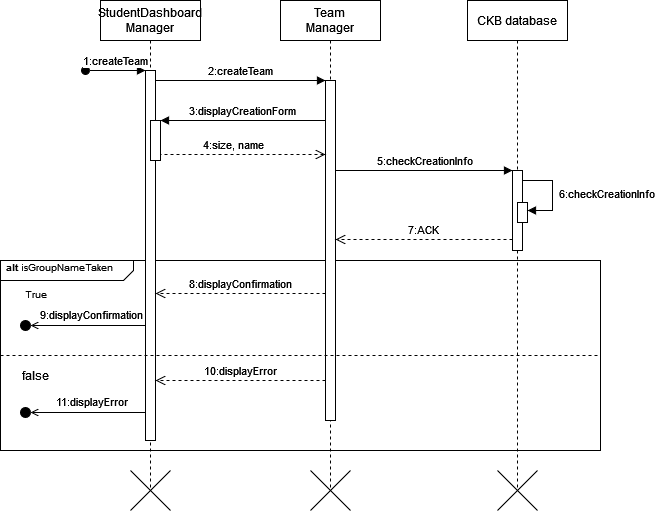
\includegraphics[width=\linewidth]{Images/sequence/Sd_teamcreation.png}
        \caption{Student create team sequence diagram}
        \label{fig:student_create_team}
    \end{center}
\end{figure}


\paragraph{Student invites another student to the team}
After the team has been created, the student can invite other students to join the team. 
The student can call the \verb|inviteStudent| function through the \verb|TeamManagerI| interface.
\verb|TeamManager| component will send a request to the \verb|StudentDashboardManager| for the email of the student to invite. 
After the student has inputed the information, the \verb|TeamManager| will check the CKB database to ensure the student is not already in a team.
Then it will send an email to the student to invite him to the team and notificate the student of the success or send an error.

\begin{figure}[H]
    \begin{center}
        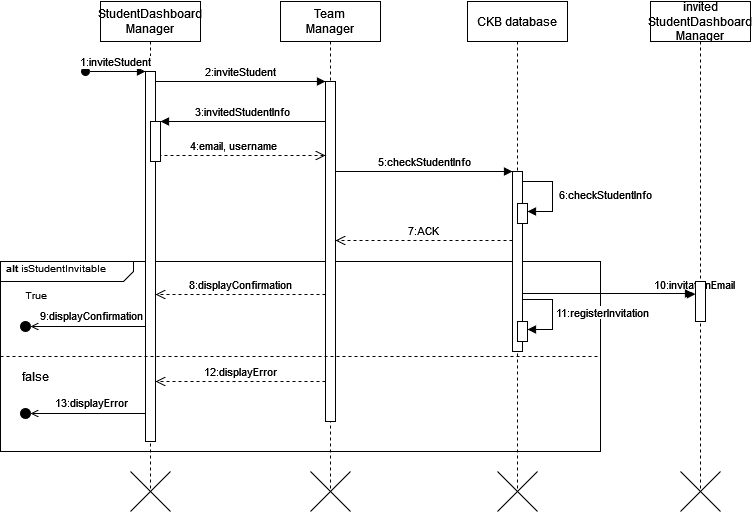
\includegraphics[width=\linewidth]{Images/sequence/Sd_invitation.png}
        \caption{Student invitation sequence diagram}
        \label{fig:student_invite}
    \end{center}
\end{figure}

\paragraph{Student accepts or rejects an invitation to join a team}
After receiving an invitation to join a team, a student can accept or reject this invitation by invoking the \verb|acceptInvitation| or \verb|rejectInvitation| function through the \verb|TeamManagerI| interface. 
The \verb|TeamManager| component processes the request, either adding the student to the team or removing the invitation from the CKB database, depending on the student's decision. 
The \verb|TeamManager| then notifies the student of the outcome. If the operation is successful, a confirmation is sent. If an error occurs, an error message is returned, allowing the student to handle the error appropriately.

\begin{figure}[H]
    \begin{center}
        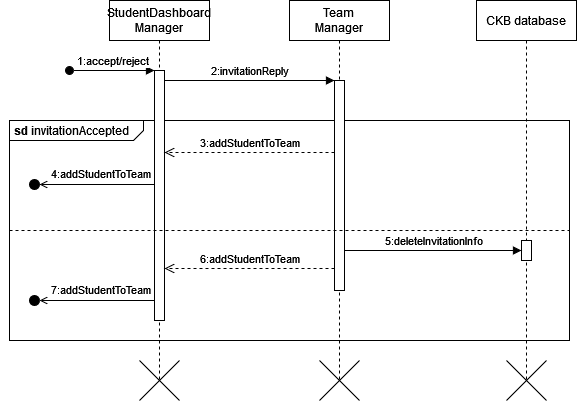
\includegraphics[width=\linewidth]{Images/sequence/Sd_invitationHandle.png}
        \caption{Student handle invite sequence diagram}
        \label{fig:student_handle_invite}
    \end{center}
\end{figure}

\paragraph{Student join a battle}
When a student, either individually or as part of a team, wishes to join a battle, they invoke the \verb|joinBattle| function from the \verb|BattleI| interface. This function requires specific parameters such as the battle ID and student or team ID. 
The \verb|BattleManager| receives the request and checks the registration deadline. If the deadline has not passed, the \verb|BattleManager| admits the student or team to the battle and updates the CKB database accordingly. A confirmation is then sent to the client. 
If the deadline has passed or if any other error occurs, an error message is returned to the client, allowing them to handle the error and provide appropriate feedback to the student.

\begin{figure}[H]
    \begin{center}
        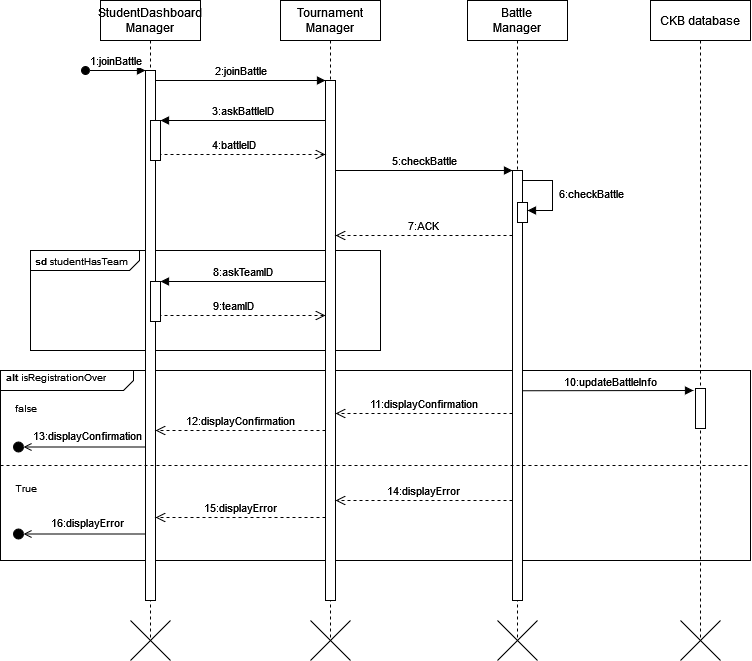
\includegraphics[width=\linewidth]{Images/sequence/Sd_joinBattle.png}
        \caption{Student join battle sequence diagram}
        \label{fig:student_join_battle}
    \end{center}
\end{figure}

\paragraph{Educator creates a tournament}
To create a tournament, the \verb|EducatorDashboardManager| invokes the \verb|createTournament| function from the \verb|TournamentI| interface. 
This function requires specific parameters such as the tournament name, number of participants, and other relevant details. The \verb|createTournament| function then passes the request to the \verb|TournamentManager| component. 
The \verb|TournamentManager| handles the creation of the tournament, including any necessary error checking, and inserts the tournament details into the database. If the tournament creation is successful, a confirmation is returned to the \verb|EducatorDashboardManager|. 
If the creation fails, an error message is returned instead, allowing the \verb|EducatorDashboardManager| to handle the error and provide appropriate feedback to the educator.

\begin{figure}[H]
    \begin{center}
        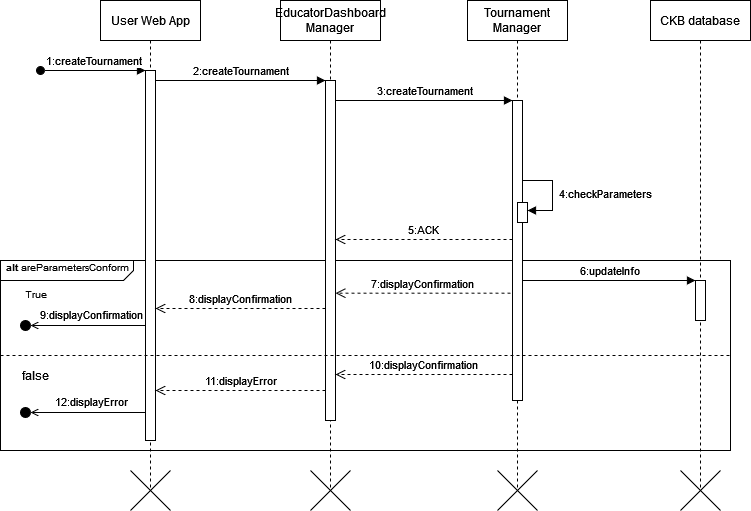
\includegraphics[width=\linewidth]{Images/sequence/Sd_createTournament.png}
        \caption{Educator create tournament sequence diagram}
        \label{fig:Educator_create_tournament}
    \end{center}
\end{figure}

\paragraph{Educator uploads a CKB}
When an educator needs to upload a CKB, they can invoke the \verb|uploadCKB| function from the \verb|BattleI| interface. This function requires specific parameters such as the CKB file and its associated metadata. 
The \verb|BattleManager| component receives the request and processes it by validating the CKB file and its metadata, and then storing them in the CKB database. 
During this process, the \verb|BattleManager| performs necessary checks, such as verifying the file format and integrity. If the operation is successful, a confirmation is sent back to the \verb|EducatorDashboardManager|. 
In case of an error, such as the file being in an incorrect format or corrupted, an error message is returned, allowing the \verb|EducatorDashboardManager| to handle the error and provide appropriate feedback to the educator.

\begin{figure}[H]
    \begin{center}
        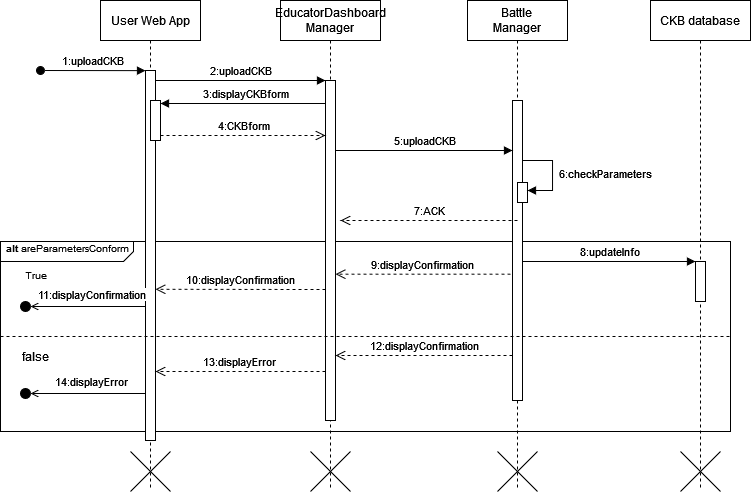
\includegraphics[width=\linewidth]{Images/sequence/Sd_uploadCKB.png}
        \caption{Educator upload ckb sequence diagram}
        \label{fig:Educator_upload_ckb}
    \end{center}
\end{figure}

\paragraph{Educator grants permission to another educator}
When an educator needs to grant permission to another educator, they can invoke the \verb|grantPermission| function from the \verb|TournamentI| interface. This function requires specific parameters such as the tournament ID and the educator ID.
The \verb|TournamentManager| component receives the request and processes it by granting the specified educator permission to manage the specified tournament.

\begin{figure}[H]
    \begin{center}
        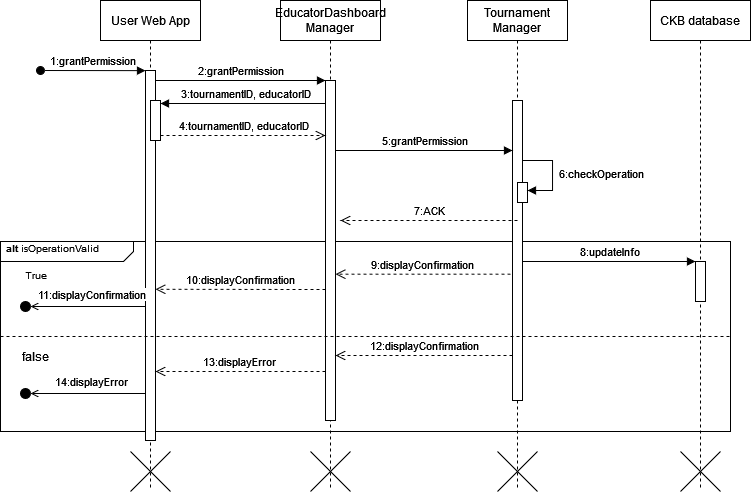
\includegraphics[width=\linewidth]{Images/sequence/Sd_grantPermission.png}
        \caption{Educator grant permission sequence diagram}
        \label{fig:Educator_grant_permission}
    \end{center}
\end{figure}


\paragraph{Educator creates a new badge}
When an educator needs to create a new bagde, they have to create new rules associated with the new badge. They can invoke the \verb|createBadge| function from the \verb|BadgeI| interface. This will required inputing the badge name, description and the rules associated with the badge.
The \verb|BadgeManager| should display a form with various pre-built rules to choose from, but the educator can also invoke the \verb|createRule| function from the \verb|GamificationRulesI| interface.
This function requires specific parameters such as the rule name, the rule description and the rule formula. The \verb|GamificationRulesManager| component receives the request and processes it by validating the rule formula and storing it in the CKB database.
During this process, the \verb|GamificationRulesManager| performs necessary checks, such as verifying the formula syntax. If the operation is successful, a confirmation is sent back to the \verb|EducatorDashboardManager|.
In case of an error, such as the formula being in an incorrect format or corrupted, an error message is returned, allowing the \verb|EducatorDashboardManager| to handle the error and provide appropriate feedback to the educator.
Once the rules are created, the \verb|BadgeManager| can create the badge and store it in the CKB database. If the operation is successful, a confirmation is sent back to the \verb|EducatorDashboardManager|.
In case of an error, such as the badge name being already used, an error message is returned, allowing the \verb|EducatorDashboardManager| to handle the error and provide appropriate feedback to the educator.

\begin{figure}[H]
    \begin{center}
        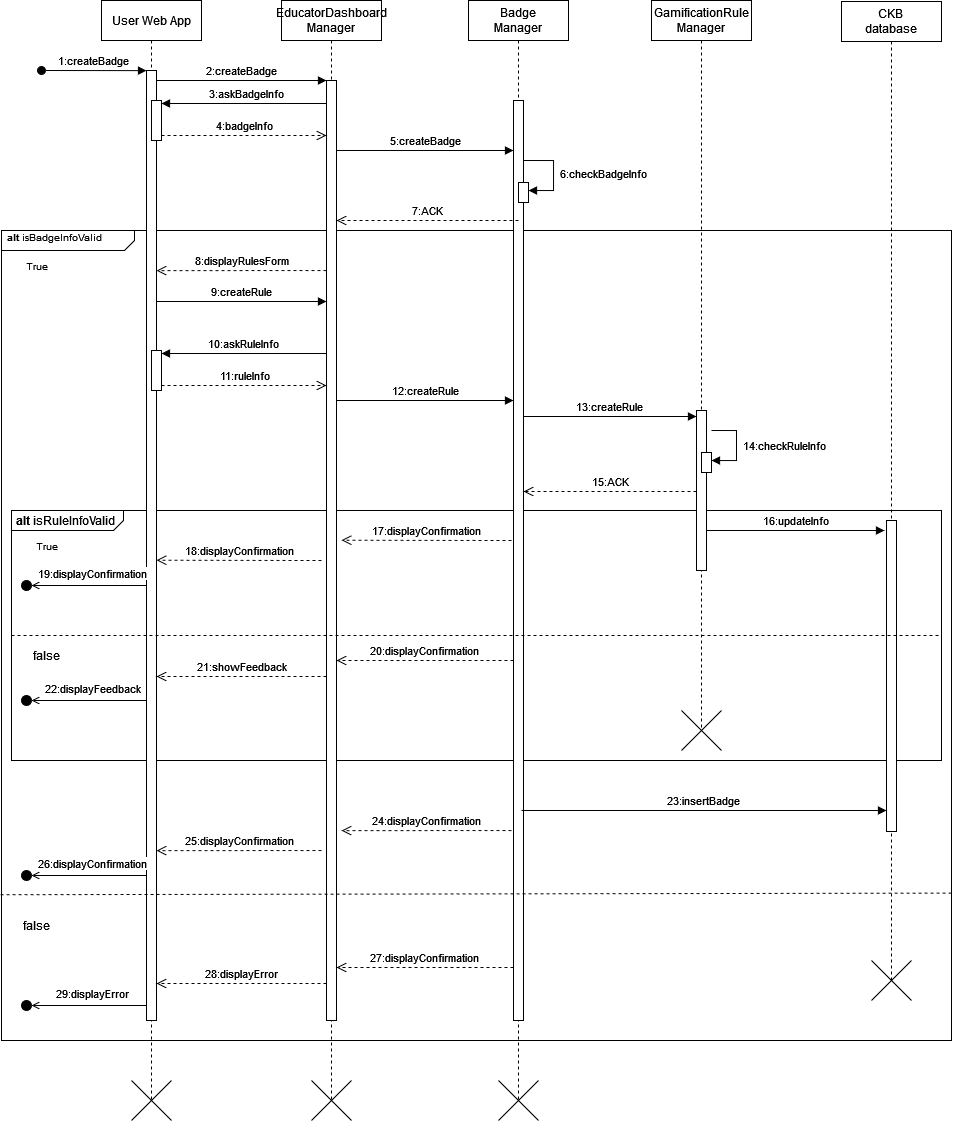
\includegraphics[width=\linewidth]{Images/sequence/Sd_badgeCreation.drawio.png}
        \caption{Educator create badge sequence diagram}
        \label{fig:Educator_create_badge}
    \end{center}
\end{figure}


\paragraph{Educator manually evaluates a team}
When an educator needs to manually evaluate a team, they can invoke the \verb|evaluateTeam| function from the \verb|BattleI| interface. This function requires specific parameters such as the battle ID and the team ID.
The \verb|BattleManager| component receives the request and processes it by evaluating the specified team and updating the CKB database accordingly. If the operation is successful, a confirmation is sent back to the \verb|EducatorDashboardManager|.
In case of an error, such as the team not existing or the battle not being closed, an error message is returned, allowing the \verb|EducatorDashboardManager| to handle the error and provide appropriate feedback to the educator.

\begin{figure}[H]
    \begin{center}
        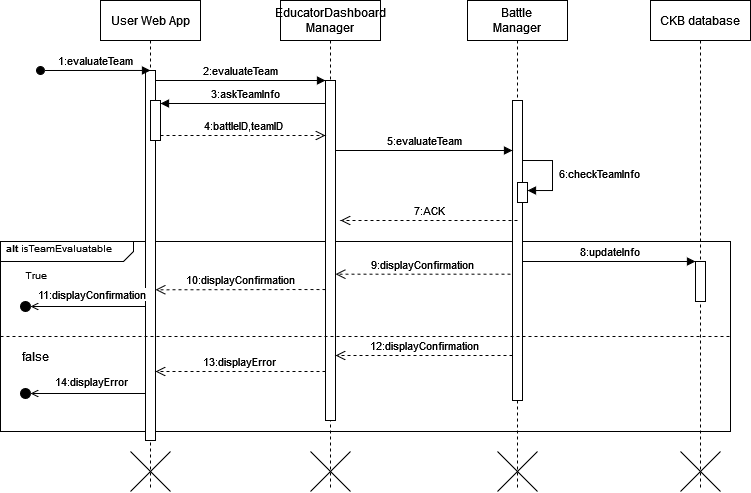
\includegraphics[width=\linewidth]{Images/sequence/Sd_manualEvaluation.png}
        \caption{Educator manually evaluate sequence diagram}
        \label{fig:Educator_manually_evaluate}
    \end{center}
\end{figure}



\paragraph{User visualize tournament rankings}
When a user wants to visualize the rankings of a tournament, they can invoke the \verb|getTournamentRankings| function from the \verb|TournamentI| interface. This function requires specific parameters such as the tournament ID.
The \verb|TournamentManager| component receives the request and processes it by retrieving the rankings of the specified tournament from the CKB database. If the operation is successful, the rankings are sent back to the client.

\begin{figure}[H]
    \begin{center}
        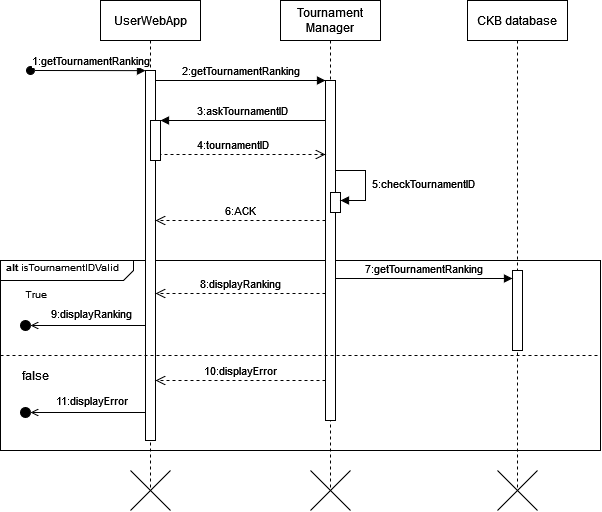
\includegraphics[width=\linewidth]{Images/sequence/Sd_seeTournamentRanking.png}
        \caption{User see tournament ranking sequence diagram}
        \label{fig:user_see_tournament_ranking} 
    \end{center}
\end{figure}


\paragraph{User visualize other users' profiles}
When a user wants to visualize the profile of another user, they can invoke the \verb|getUserProfile| function from the \verb|UserManagerI| interface. This function requires specific parameters such as the user ID.
The \verb|UserManager| component receives the request and processes it by retrieving the profile of the specified user from the CKB database. If the operation is successful, the profile is sent back to the client.


\begin{figure}[H]
    \begin{center}
        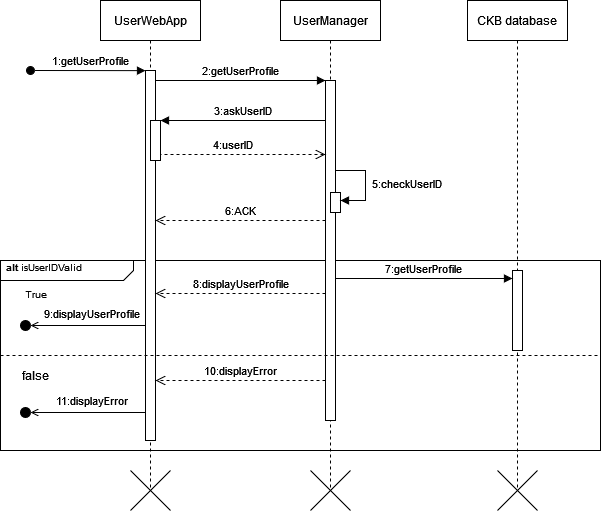
\includegraphics[width=\linewidth]{Images/sequence/Sd_seeUserProfile.png}
        \caption{User see profile sequence diagram}
        \label{fig:User_see_profile}
    \end{center}
\end{figure}
\newpage

\section{Selected architectural styles and patterns}

In this section are shown the most relevant architectural design choices, with also the explanation of their role and their advantages.

\textbf{3 Tier Architecture}\newline
N-tier architecture refers to the structure of a software application divided into multiple tiers. 
A tier is a layer of the application that operates on its own infrastructure or server. 
In particular, we decided to implement a 3-tier architecture. The tiers are: presentation, logic, and data tier.\newline
Presentation tier → It presents information to users and receive user inputs\newline
Logic tier → It handles business logic and application processing logic. It’s responsible for processing user requests, 
applying business rules, and managing the flow of data between the presentation and data tier\newline
Data tier → It manages the storing and retrieving of the data. It handles data persistence and integrity too\newline
The advantages of using this type of architecture revolve around its scalability, ease of management, and flexibility and security. 
If we need to add more resources to a specific tier or modify it, we can do so without affecting the other tiers. Moreover, we can secure each 
of the three tiers separately using different methods and techniques, based on the security needed for the specific tier

\textbf{WebSocket with Pub/Sub Pattern}\newline
The WebSocket protocol provides a full-duplex communication channel over a single TCP connection. 
This means that data can be sent and received at the same time, allowing for real-time communication between the client and the server.
The Publish/Subscribe pattern is a messaging pattern where senders (publishers) categorize messages into classes without knowing which 
subscribers (if any) there might be. Similarly, subscribers express interest in one or more classes, and only receive messages that are of interest, 
without knowing which publishers there are
When combined, WebSocket and Pub/Sub can be a powerful tool for real-time web applications. Regarding the CKB specifically:\newline
1. Publishing → when an event occurs in CKB (e.g., a new battle is created, a score is updated,…), the server publishes a message about this event. 
The message is categorized based on the type of event (e.g., “New Battle”, “Score Updated”,…)\newline
2. Subscribing → Clients (users of CKB) subscribe to the types of events they’re interested in. 
For example, a student might subscribe to “New Battle” events to be notified when a new battle is created.\newline
3. Real-Time Updates → Because the communication is happening over WebSocket, these messages can be pushed from the 
server to the client in real-time. As soon as a new message is published, all clients subscribed to that type of event will receive the message.\newline
4. Scalability → The Pub/Sub pattern allows for scalability. As the number of users (subscribers) and events (publishers) increases, 
the system can continue to function efficiently.\newline
This combination of WebSocket and Pub/Sub can provide a dynamic, real-time user experience for CKB, making it more engaging and responsive for its users.

\textbf{Worker Pooling}\newline
Worker pooling refers to a pattern where a set of initialized “workers” (threads, processes, or any kind of parallel-executing entities) 
are kept ready to perform a certain kind of task. In the context of CKB, worker pooling can help to improve the performance and 
responsiveness of your server by reusing workers instead of creating new ones for each request. This can be particularly helpful in 
a high-load scenario where new requests are coming in faster than the server can create new workers. 
Moreover, thanks to the presence of the reverse proxy, we can obtain a balanced load cross the network. 
Infact, a reverse proxy can distribute incoming requests to multiple server replicas. 
This is done to achieve evenly distributed load across the servers replica, 
preventing any single server from becoming a bottleneck. 
Each replica would have its own worker pool to handle the requests it receives

\textbf{Microservices}\newline
The application uses a suite of small services, instead of being monolithic, 
each running in its own process and communicating with the other microservices. 
To communicate between each other, microservices can exploit an event-driven paradigm (like publisher and subscriber). 
Moreover, other design choice must be taken into consideration, for example to achieve resiliency. 
One suggestion could be to utilize a Circuit Breaker to inhibit all those microservices that are failing repeatedly. 
In the specific context of CKB, this could be momentarily debilitating some functions of the platform, 
such as the possibility to visualize the leaderboard of a Tournament or adding members to a team. 
This way, the platform itself can keep running, and maintenance can be executed on the faulty microservices to bring them back up as quickly as possible

\textbf{Database: NoSQL with SQL}\newline
In the context of CodeKataBattle (CKB), the use of two different databases, a NoSQL database (MongoDB) and a SQL database (MySQL), 
is a strategic decision aimed at leveraging the strengths of both types of databases to efficiently manage and access data.\newline
Let’s look at the strength of using a NoSQL database.\newline
Scalability → NoSQL databases are more scalable than traditional relational databases. 
They can spread out the data storage and computing processes over a cluster of computers. 
This allows for almost unlimited growth as increasing capacity simply requires adding more computers to the cluster.\newline
Flexible Data Model → Unlike relational databases, NoSQL databases can easily store and combine any type of data, both structured and unstructured. 
They can dynamically update the schema to evolve with changing requirements without any interruption or downtime to an application.\newline
Resilience → With NoSQL, data is distributed across multiple servers and regions, so there is no single point of failure. 
As a result, NoSQL databases are more stable and resilient, with continuous availability and zero downtime.\newline
Given these characteristics, a NoSQL database is suitable for storing most of the data from our CKB platform, like users, 
educators, tournaments’ results, badges, notifications, etc. Infact, the platform should be able to deal with collecting a 
big number of data and storing them for later retrieval. We aspect that the system won’t perform many queries on the data stored in the NoSQL database. 
Thus, it’s main functionality is to store long time data to ensure that every user can check out past events without problem 
(so for example, a user that wants to see the leaderboard of a Tournament ended months before, or when visiting the profile of another user)\newline
On the other hand, we have the SQL database. While the system exploits the NoSQL database mostly for storing tons of data over time, 
we are going to use the SQL database to store the data for which we expect a high number of queries will be performed. This is the case of an ongoing Tournament. 
In fact, lot’s of user will access the battles of the tournament, push their solutions, form teams, and so on. 
This requires the system to perform a high number of data retrieval from the database, and using a SQL database it ensures smooth operation. 
Therefore, we will store data like Battles, teams, and Tournaments in the SQL database. Once a Tournament is closed, 
we could free the memory of the SQL databases after updating the NoSQL one. This will allow to avoid saturation of the database and faster retrieval of data.\newline
The entity ‘Tournament’ is shared between both databases, necessitating synchronization to ensure data consistency. 
The decision between updating the NoSQL when a specific Tournament ends or while it is still on depends on the capacity of the system and the stress it can undergo. 
As a best practice, periodic synchronization between the SQL database and the NoSQL database while a Tournament is on are suggested.

\section{Other Design decisions}

\textbf{Firewall}\newline
A firewall is a network security system that monitors and controls incoming and outgoing traffic based on predetermined security rules. 
The firewall sits between the CKB’s network and the larger internet, examining all network traffic and blocking any 
that doesn’t meet its configured security rules. This can help protect CKB from various types of attacks, 
such as SQL injection, cross-site scripting and other exploits that could take advantage of vulnerabilities in the web application. 
Moreover, a firewall can prevent unauthorized data from leaving the web application, adding an extra layer of data protection. 
This is particularly important for a platform like CKB, which might handle sensitive data such as coding challenge solutions and users’ info. 
The firewall must be configured to allow WebSocket traffic, which is used for real-time updates in CKB.

\textbf{Reverse Proxy}\newline
A reverse proxy is a server that sits between client devices and a web server, forwarding client requests to the web server and returning the server’s 
responses back to the clients. In CKB, the reverse proxy plays a crucial role in managing and directing network traffic to multiple server replicas. 
The reverse proxy receives client requests and intelligently distributes them across multiple server replicas, each equipped with its own worker pool. 
This distribution is done in a manner that ensures an evenly balanced load across the network, preventing any single server from becoming a bottleneck. 
This is particularly beneficial in high-load scenarios where numerous requests are coming in simultaneously.\newline
Moreover, the reverse proxy provides an additional layer of abstraction and control to ensure smooth flow of network traffic between clients and servers. 
It can provide additional features like SSL termination, HTTP/2 support, caching, and more. This not only enhances performance but also adds a layer of security, 
shielding the servers from direct exposure to the internet.\newline
In addition, the reverse proxy can provide other benefits such as masking the internal structure of the backend network, providing a single point of entry into the system, 
and simplifying routing and network configuration. It can also provide resilience by detecting failure of a server replica and redirecting traffic to other healthy replicas


\textbf{Model-View-Controller (MVC)}\newline
The Model-View-Controller (MVC) is a design pattern widely used in software development, particularly in object-oriented programming and web application. 
It separates an application into three main logical components: the Model, the View, and the Controller\newline
Model → The Model contains the methods for accessing data useful to the application. 
In CKB, this could include data related to users, battles, tournaments, scores, etc. The Model directly manages the data, logic, and rules of the application\newline
View → The View is responsible for displaying data to the user and managing the interaction between the user and the underlying infrastructure. 
In CKB, this could include the user interfaces for viewing and joining battles, viewing scores, etc.\newline
Controller → The Controller receives user commends through the View and reacts by performing operations that can affect the Model and 
generally lead to a change of state in the View. In CKB, this could include operations like creating a new battle, etc.\newline
The MVC pattern simplifies the code of applications by logically separation concerns. 
This separation allows developers to focus on one aspect of the software at a time, making the code easier to understand, maintain, and expand. 
It also improves efficiency by allowing different parts of the code to be developed and tested independently.

\textbf{Factory pattern}\newline
The factory pattern is a creational design pattern that provides an interface for creating objects in a superclass, but allows subclasses to 
alter the type of objects that will be created. In the context of CodeKataBattle (CKB), the Factory pattern can be effectively used for badge creation, 
providing a robust and flexible solution for creating different types of badges. It simplifies the badge creation process, 
makes it easy to add new types of badges, and decouples the badge creation logic from the resto of the application

\textbf{Decorator pattern}\newline
The decorator pattern is a design pattern that allows behavior to be added to an individual object, dynamically, without affecting the behavior of other instances of the same class. 
In the context of CKB, the decorator pattern can be effectively used for the score system. 
The base Score component defines the interface for objects that can have responsibilities added to them dynamically. 
Decorators wrap a Score component and define a new behavior for the methods that calculate the score.\newline
The Decorator patten provides a flexible alternative to subclassing for extending functionality